\documentclass[a4paper, 11 pt, article, accentcolor=tud7b]{tudreport}

\usepackage[utf8]{inputenc}
\usepackage{amsmath}
\usepackage{placeins}
\usepackage{graphicx}

\title{CNuVS Exercise 7}
\author{Nils Rollshausen, Daniel Drodt}
\subtitle{Nils Rollshausen, Daniel Drodt}

\begin{document}
	\maketitle
	\section{Flow Control}
	\subsection*{a) Purpose}
	Flow control exists to protect receiving network nodes from being overrun with more traffic than they can handle.
	  
	\subsection*{b) Problems}
	One problem that can occur when providing flow control on the transport layer is that the packet indicating that the receiving node is unable to process more traffic takes some time to arrive at the sending node which may continue sending packets that cannot be processed at the receiving node. Another problem is that traffic may degrade into a choppy stop-and-go where the receiving node alternates between being overloaded and idle while waiting for control messages to propagate.
	
	\subsection*{c) Rate-based vs. Window-based}
	Rate-based flow control relies on the receiver to actively indicate the maximum transfer rate it can support by sending control packets to the sender periodically. Window-based flow control allows senders to have a previously agreed on number of packets in flight (unacknowledged) simultaneously. When this number is exceeded, the sender has to wait for previous packets to be acknowledged before sending new ones. In its acknowledgements, the receiver may indicate a change in the window size. \\
	In a high-speed network, the amount of data sent until a control packet makes its way from receiver to sender may be very large - therefore, to prevent large amounts of dropped packages, it is probably advisable to use window-based flow control on such networks.

  \newpage

	\section{TCP Flow Control}

	\begin{figure}[h]
		\centering
		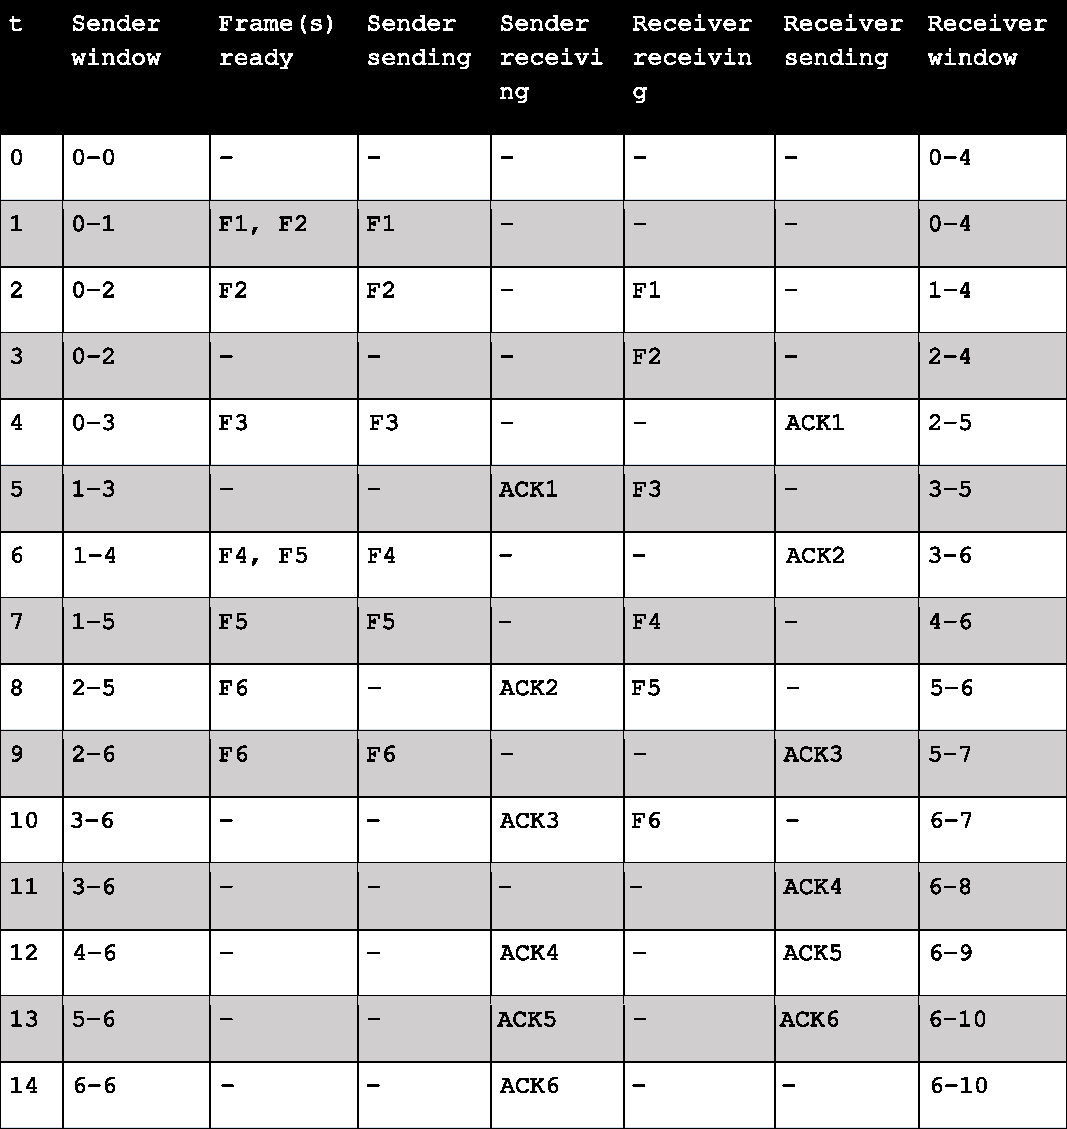
\includegraphics[]{table1.pdf}
	\end{figure}

	\FloatBarrier
	
	\section{Sliding Window Protocols}
	
	\textit{See following page}

	\begin{figure}[h]
		\centering
		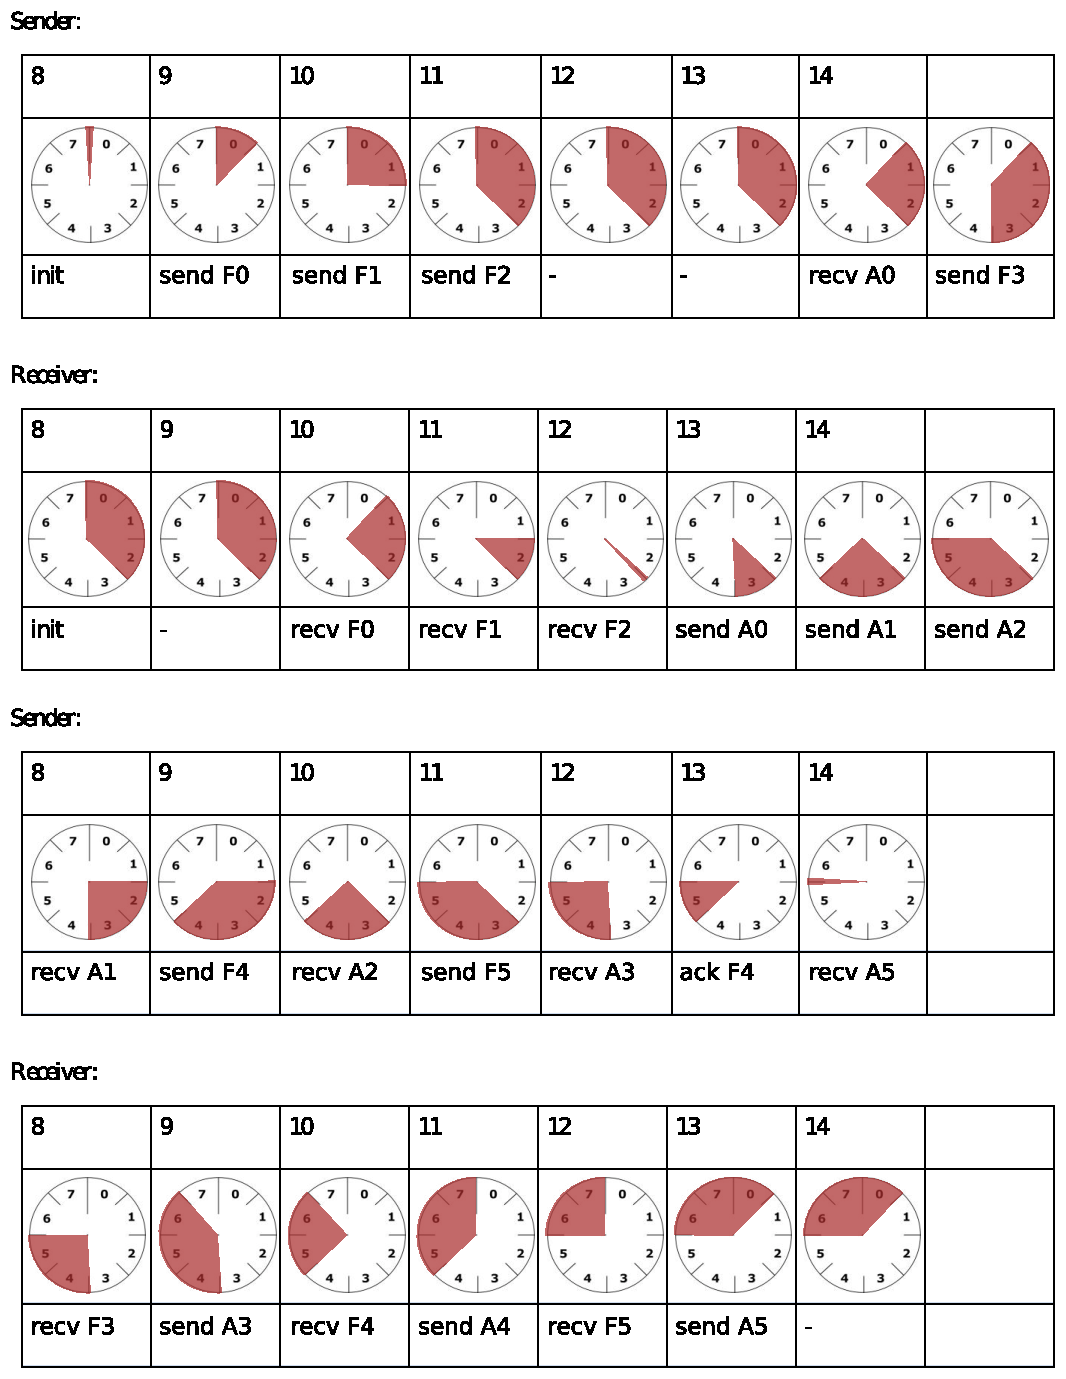
\includegraphics[]{table2.pdf}
	\end{figure}
	
\end{document}
